\thispagestyle{empty}

\begin{center}
  \theauthor
\end{center}

\medskip
\begin{center}
  \textbf{\MakeUppercase{\thetitle}}
\end{center}

\medskip
\noindent {\small Este Trabalho de Conclusão de Curso foi julgado 
adequado para a obtenção do título de Bacharel em Engenharia Eletrônica
e aprovado em sua forma final pelo Curso de Graduação em Engenharia 
Eletrônica.}

% Versão pra impressão (sem assinaturas)

% Para melhor qualidade scanear (ou então após usar algum editor de imagens) cada assinatura separadamente, como exemplo a Figura assinatura01.png

\begin{center}
	
\includegraphics[width=5cm]{fig/sig-rangel.jpg}\\
	Prof. Fernando Rangel de Sousa, Ph.D.\\
	{\footnotesize Coordenador do Curso}
\end{center}
\medskip
\textbf{Banca examinadora:}
\bigskip
\begin{center}
	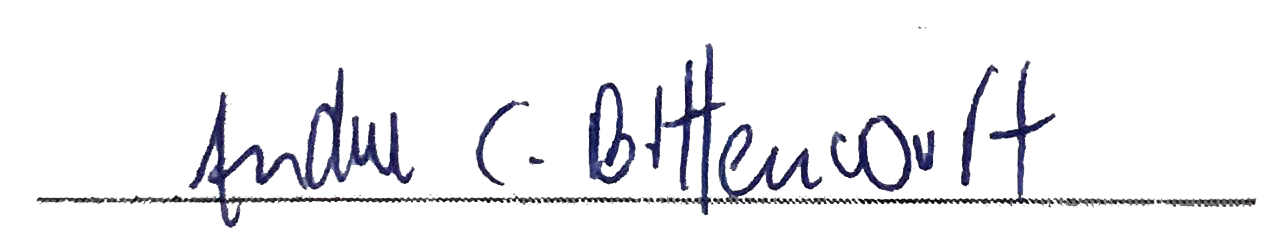
\includegraphics[width=5cm]{fig/sig-andre.png}\\
	\theadvisor, Ph.D.\\
	{\footnotesize Orientador}\\
	{\footnotesize Neoway Business Solutions}
\end{center}
\begin{center}
	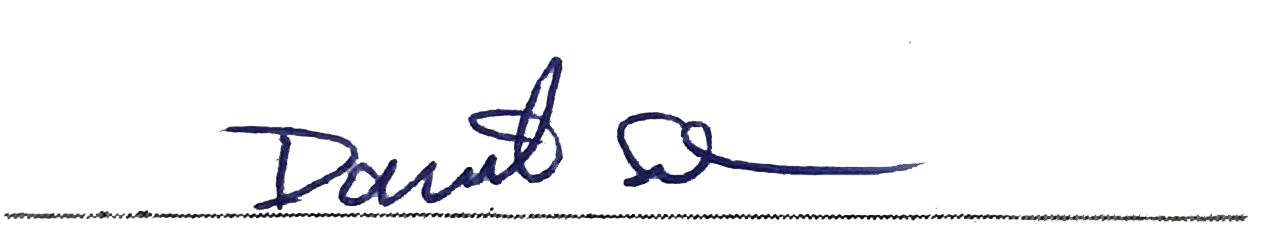
\includegraphics[width=5cm]{fig/sig-danilo.png}\\
	Prof, Danilo Silva, Ph.D.\\
	{\footnotesize Universidade Federal de Santa Catarina}
\end{center}
\begin{center}
	
\includegraphics[width=5cm]{fig/sig-penha.png}\\
	\thecoadvisor, Ph.D.\\
	{\footnotesize Co-Orientador}\\
	{\footnotesize Neoway Business Solutions}
\end{center}
\begin{center}
	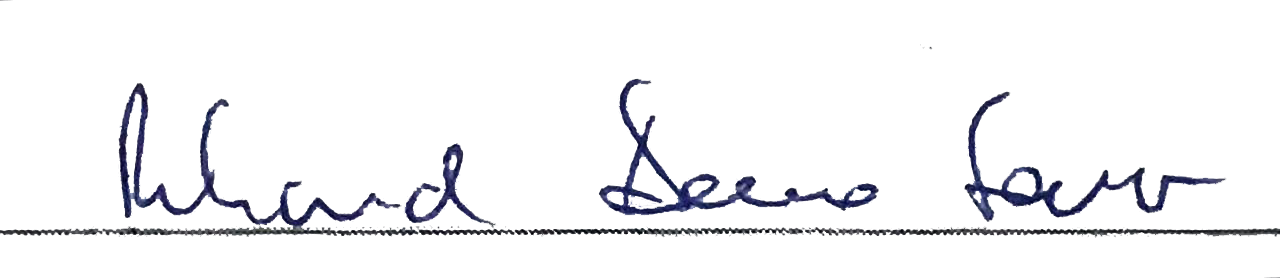
\includegraphics[width=5cm]{fig/sig-richard.png}\\
	Prof. Richard Demo Sousa, Ph.D.\\
	{\footnotesize Universidade Federal de Santa Catarina}
\end{center}
\medskip